\section{Results and Discussion}


\begin{figure}
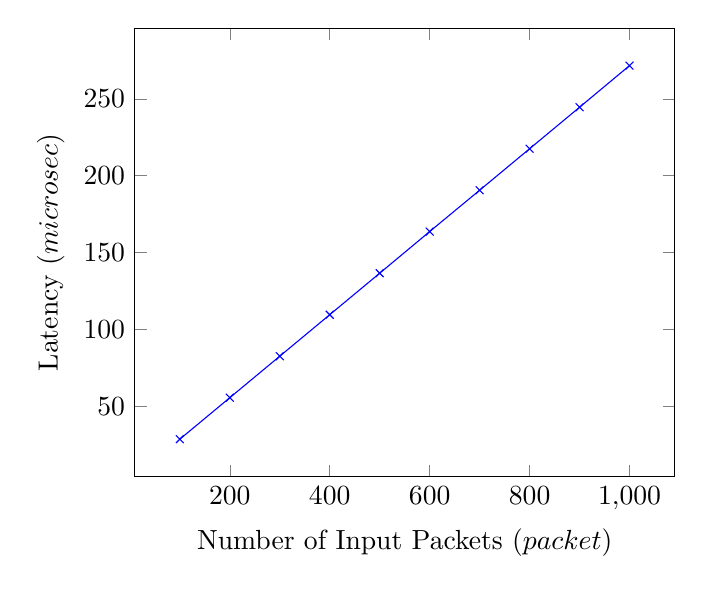
\begin{tikzpicture}
	\begin{axis}[
		xlabel=Number of Input Packets $(packet)$,
		ylabel=Latency $(microsec)$]
	\addplot[color=blue,mark=x] coordinates {
		(100,28.5)
		(200,55.5)
		(300,82.5)
		(400,109.5)
		(500,136.5)
		(600,163.6)
		(700,190.5)
		(800,217.5)
		(900,244.5)
		(1000,271.6)
	};
	\end{axis}
\end{tikzpicture}
\caption{Relationship between latency and the number of input packets} \label{fig:plot1}
\end{figure}


\begin{figure}
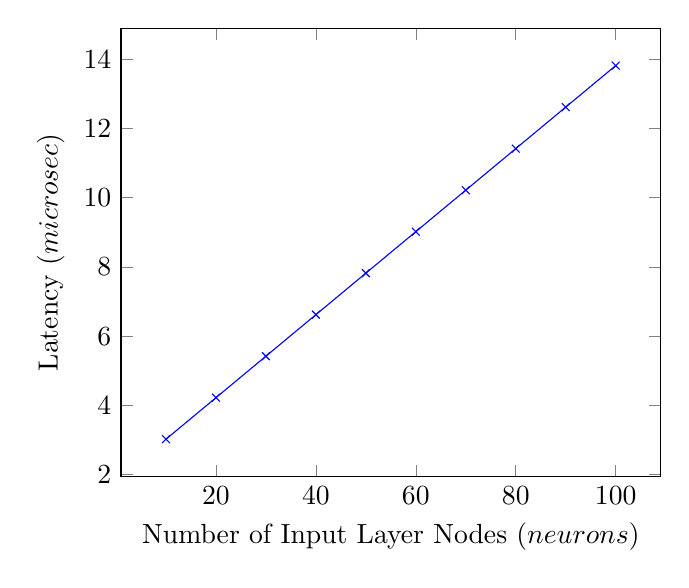
\begin{tikzpicture}
	\begin{axis}[
		xlabel=Number of Input Layer Nodes $(neurons)$,
		ylabel=Latency $(microsec)$]
	\addplot[color=blue,mark=x] coordinates {
		(10,3.02)
		(20,4.22)
		(30,5.42)
		(40,6.62)
		(50,7.82)
		(60,9.02)
		(70,10.22)
		(80,11.42)
		(90,12.62)
		(100,13.82)
	};
	\end{axis}
\end{tikzpicture}
\caption{Relationship between latency and the number of nodes in the input layer} \label{fig:plot2}
\end{figure}
